Im dritten Teil der Arbeit wird die im zweiten Teil entwickelte DSL in eine bestehende medizinische Dokumentationssoftware eingebunden.

Die Implementierung der FXL ist eine eigenständige Java-Bibliothek und damit unabhängig vom Zielsystem. Um die Bibliothek zu verwenden, muss evaluiert werden, wie und wo die Schnittstellen integriert werden können und wie die Interaktion mit dem Endbenutzer des Systems gestaltet wird.  

Zuerst wird das Studiensystem SPICS beschrieben, um dem Leser der Arbeit eine Übersicht über das System zu bieten. Es soll helfen, das not\-wen\-dige Verständnis für den Nutzen der FXL zu erzeugen. Danach werden die einzelnen Aspekte und Überlegungen bei der Integration vorgestellt.

\chapter{Systembeschreibung}
\label{chapter_systembeschreibung}

Dieses Kapitel erläutert den Aufbau der Dokumentationssoftware SPICS, um ein Verständnis für die Anwendung der Form Expression Language in der Implementierung herzustellen. Neben der Beschreibung des technischen Aufbaus werden auch die konkreten Anwendungsfälle der FXL erklärt, um nachvollziehen zu können, an welchen Stellen in den Workflow eingegriffen wird.


\section{SPICS}

SPICS (Secure Platform for Integrating Clinical Services) ist ein Projekt der  Forschungsgruppe Industrial Software der TU Wien. Die Software ist eine Webanwendung, die Krankenhäusern, Ärzten und anderen Spezialisten -- unter Berücksichtigung des Datenschutzgesetzes -- den gemeinsamen Zugriff auf Daten für medizinische Studien er\-mög\-licht. 

Die SPICS Plattform bietet die Möglichkeit, für verschiedene medizinische Fachbereiche bzw. Anforderungen individuelle Eingabemasken zu erstellen. Dafür können aus unterschiedlichen Formularfeldern flexibel benutzerdefinierte Formulare erstellt werden. Weitere Features sind der Import und Export der gesammelten Studiendaten, um diese mit externen Statistik-Tools auszuwerten. Dabei ist zu beachten, dass die Anonymität der Patienten und Studienteilnehmer gesichert ist, da die medizinischen Daten nur pseudonymisiert abgelegt werden.


\section{Workflow}
\label{section_systembeschreibung_workflow}

Um die Integration in das Dokumentationssystem zu verstehen, werden zuerst die wichtigsten Anwendungsfälle erörtert, um zu veranschaulichen, wo die DSL die Arbeit mit den Daten erleichtern kann. Zuerst wird der typische Ablauf anhand eines Beispiels durchgespielt, um danach zu erläutern, wo die FXL den Workflow verbessern kann.

SPICS enthält ein umfassendes Rollen- und Berechtigungssystem. Die für diese Arbeit essentiellen Rollen sind jene des Administrators und des Contributors. Administratoren sind berechtigt, Formulare zu erstellen und zu bearbeiten. Contributoren sind hingegen jene Benutzer, die Daten in die Formulare eingeben.

\subsection{Workflow anhand eines Beispiels}
\label{subsection_workflow_beispiel}


Um den typischen Ablauf zu verdeutlichen, werden die maßgeblichen Anwendungsfälle für ein beispielhaftes Formular angeführt. Im darauf folgenden Abschnitt wird eruiert, wo die FXL in diesen Ablauf eingreift, um den Endanwender bei der Eingabe der medizinischen Daten zu unterstützen.

Natürlich enthält ein so aufwändiges System wie SPICS neben dem \mbox{hier} vorgestellten auch zahlreiche weitere Workflows, etwa für Datenexport und -import, Benutzerverwaltung, Konfiguration und Terminverwaltung. Auf diese soll hier jedoch nicht eingegangen werden, um den Focus auf das Thema der Arbeit nicht zu verlieren.

Der Workflow soll am Beispiel eines Formulars gurchgegangen werden, in dem die Veränderung des Body-Mass-Index (BMI) eines Patienten dokumentiert wird. Ein Arzt (bzw. aus Software-Sicht: der Endanwender) soll also in der Lage sein, den BMI eines Patienten an verschiedenen Tagen zu dokumentieren. Abbildung \ref{abb_workflow_formular_ausfuellen} auf Seite \pageref{abb_workflow_formular_ausfuellen} zeigt das fertige Formular, in das die Daten eingegeben werden können.

Das in den folgenden Schritten erstellte Formular soll im gesamten zweiten Teil der Arbeit als Beispiel dienen, da es einerseits einfach nachzuvollziehen ist und andererseits einige grund\-sätz\-liche Konzepte und Überlegungen beinhaltet, die im weiteren Verlauf der Arbeit erläutert werden\footnote{vgl. Abschnitt \ref{implementierung_dsl_eingabe}  \nameref{implementierung_dsl_eingabe} sowie Abschnitt \ref{implementierung_daten_eingabe} \nameref{implementierung_daten_eingabe}}.

\subsection{Use Cases}

\subsubsection{Erstellen eines neuen Formulars}

Der erste Schritt im Workflow ist das Erstellen eines neuen Formulars. Es ist zuerst ein Titel zu vergeben, sowie einzustellen, ob das Formular pro Patient einmal oder mehrmals ausfüllbar ist. Diese Unterscheidung ist not\-wen\-dig, da manche Daten nur einmal zu erheben sind (z.B. Stammdaten, oder Daten zur Geburt eines Patienten). Oft ist es allerdings auch not\-wen\-dig (wie im oben beschriebenen Beispiel), ein Formular für einen Patienten mehrmals auszufüllen, etwa um einen zeitlichen Verlauf zu dokumentieren.
 
\begin{figure}[h]
\begin{center}
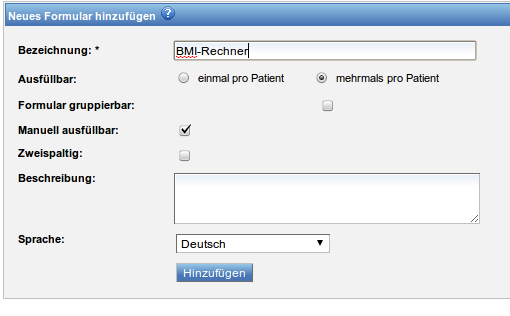
\includegraphics[scale=0.5]{figures/workflow_neues_formular}
\caption{Erstellen eines neuen Formulars}

\label{abb_workflow_neues_formular}
\end{center}
\end{figure}

Zu\-sätz\-lich können auch weitere Parameter angegeben werden (Abbildung \ref{abb_workflow_neues_formular}), die beispielsweise das Layout oder die Sprache betreffen. Diese Einstellungen haben allerdings für das Beispielformular keine Relevanz.

Das Ergebnis dieses Schrittes ist ein leeres Formular, das nun mit einer beliebigen Anzahl und Anordnung von Formularelementen gefüllt werden kann.

\subsubsection{Editieren eines Formulars}

Wenn ein Formular neu erstellt wurde (bzw. wenn es bereits existiert oder importiert wurde) kann es editiert werden. Darunter wird das Anlegen, Verändern und Löschen von Formularelementen verstanden. Zu\-sätz\-lich werden Formularelemente in Gruppen zusammengefasst, um eine übersichtliche Struktur zu schaffen.

Manche Formularelemente können mit einfachen Constraints belegt werden. So kann bei einem Datumsfeld der Datumsbereich (von-bis) ausgewählt werden. Bei Textfeldern kann der Datentyp insofern festgelegt werden, als dass zwischen \emph{Text}, \emph{Ganzzahl} und \emph{Kommazahl} unterschieden wird. Bei den beiden Letzteren ist wiederum ein Constraint möglich, der den Wertebereich einschränkt. Außerdem kann für jedes Formularelement festgelegt werden, ob es ein Pflichtfeld ist.

Für das Beispielformular wird zuerst eine Gruppe mit dem Namen `BMI-Rechner` erstellt. In dieser Gruppe werden nun drei Textfelder
für das Kör\-per\-ge\-wicht, die Kör\-per\-grö\-ße und den BMI angelegt. Zu\-sätz\-lich wird noch eine Checkbox mit dem Titel `Adipositas` hinzugefügt.

\subsubsection{Auswählen eines Patienten}

Der nächste Schritt ist die Auswahl eines Patienten, für den das Formular ausgefüllt werden soll. Hier findet ein Wechsel der Rolle des Benutzers vom Administrator zum Contributor statt. Waren für die bisherigen Schritte Berechtigungen zum Erstellen und Editieren von Formularen not\-wen\-dig, so ist ab nun lediglich die Berechtigung zum Ausfüllen der Formulare erforderlich. 

Zunächst wird ein Patient anhand seines Synonyms aus der Liste aller Patienten ausgewählt. Auf der Übersichtsseite für einen Patienten sind alle bereits ausgefüllten Formulare aufgelistet. Soll ein neues Formular hinzugefügt werden, muss der Name des Formulars ausgewählt werden. 

\subsubsection{Ausfüllen eines Formulars}

\begin{figure}[h]
\begin{center}
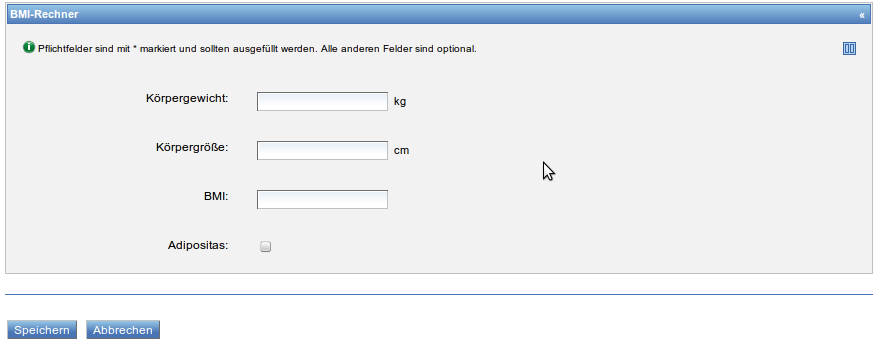
\includegraphics[scale=0.5]{figures/workflow_formular_ausfuellen}
\caption{Ausfüllen des neuen Formulars}

\label{abb_workflow_formular_ausfuellen}
\end{center}
\end{figure}

Wurde auf der Übersichtsseite eines Patienten das Formular `BMI-Rechner` ausgewählt, erscheint nun das in den vorigen Schritten erstellte Formular (Abbildung \ref{abb_workflow_formular_ausfuellen}). Der Endanwender kann nun die ent\-sprech\-enden Daten in die dafür vorgesehenen Felder eingeben. Der BMI muss hier mithilfe eines Taschenrechners oder Tools berechnet werden. Ist sein Wert größer 30, so handelt es sich laut WHO um Fettleibigkeit (Adipositas)\footnote{ vgl. \cite{Who00} }. In diesem Fall sollte die Checkbox `Adipositas` angeklickt werden.



\section{Architektur und Technologien}

Dieser Abschnitt enthält einen Überblick über die Softwarearchitektur und die verwendeten Technologien, um die Integration der Form Expression Language aus technischer Sicht nachvollziehen zu können.


\subsection{Architektur}

Die Architektur von SPICS ist als klassische 3-Tier Applikation mit gra\-phisch\-er Benutzeroberfläche, Programmlogik und Datenzugriffsschicht ausgeführt (Abbildung \ref{abb_spics_architektur}). 

\begin{figure}[h]
\begin{center}
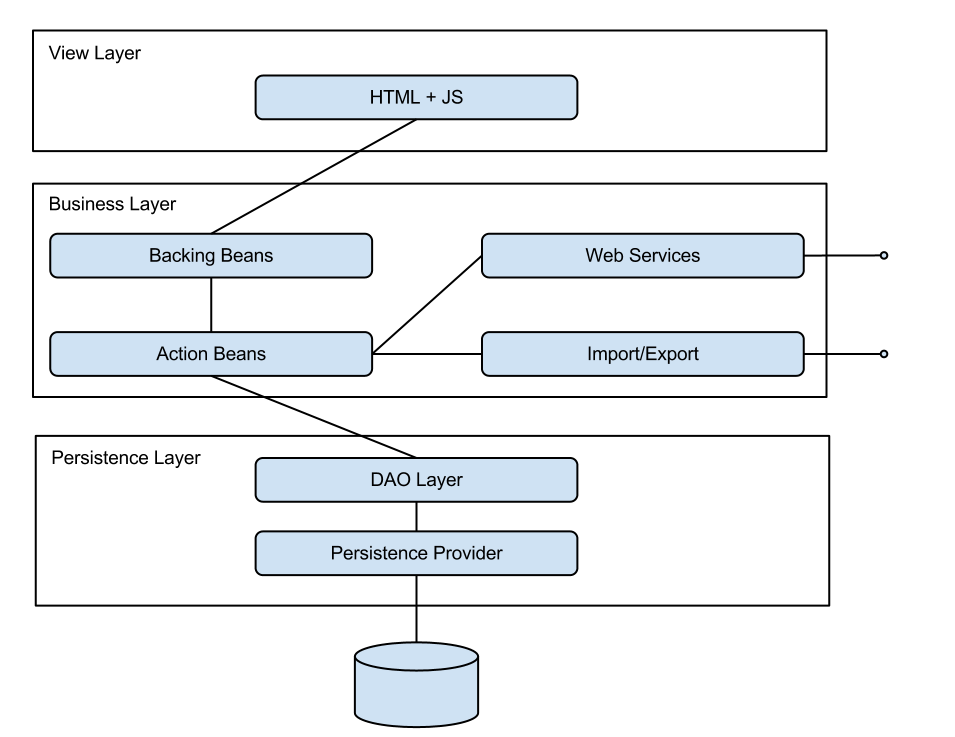
\includegraphics[scale=0.4]{figures/spics_architektur_neu}
\caption{Übersicht über die 3-Tier Architektur}

\label{abb_spics_architektur}
\end{center}
\end{figure}

Die Benutzerschnittstelle ist eine Webapplikation, die auf die Backing Beans der Logikschicht zugreift. Unterstützt wird die GUI durch Java\-Script-basierte Widgets wie z.B. Date Picker. Wo möglich bzw. sinnvoll werden AJAX-Calls verwendet, um den Workflow flüssiger zu gestalten.

Der Kern der Software besteht aus Komponenten, die die Programmlogik enthalten. Diese sind einerseits Backing Beans, deren Attribute an die Benutzerschnittstelle gebunden werden, andererseits Action Beans, in denen Daten verarbeitet werden. Zu\-sätz\-lich bietet die Software auch noch eine Webservice-Schnittstelle und Komponenten zum Import und Export von Formularen und medizinischen Daten.

Die Komponenten der Logik-Schicht greifen auf die darunter liegende Datenbank über Data Access Objects (DAOs). Das Datenmodell des Systems wird über objektrelationales Mapping auf die Tabellen der relationalen Datenbank abgebildet.



Eine zusätzliche Besonderheit von SPICS ist die Trennung der persönlichen Patientendaten von den Behandlungsdaten. Diese örtliche Trennung ist not\-wen\-dig, um den Datenschutz der Patienten zu gewährleisten. Das Zusammenführen der perönlichen Daten mit den medizinischen Daten erfolgt erst im Browser des Benutzers. Auf diese Eigenschaft wird hier nicht weiter eingegangen, da sie für die Aufgabenstellung nicht relevant ist. Sie soll aber trotzdem erwähnt werden, da dies ein Key-Feature von SPICS darstellt.

\subsection{Technology Mapping}

Der Kern der Dokumentationssoftware SPICS ist als Java Enterprise Applikation, basierend auf dem Framework Seam ausgeführt. Als Applicationserver wird der JBoss AS verwendet. Auf die darunterliegende PostgreSQL Datenbank wird mittels Hibernate als ORM Mapper zugegriffen.

Verwendete Technologien des Systems:

\begin{itemize}
	\item Java 6
	\item PostgreSQL
	\item JBoss AS 5.1.0.GA
	\item Seam 2.2
	\item JSF 1.2
\end{itemize}



\chapter{Integration}


Im folgenden Kapitel werden die einzelnen Themen der Integration der Form Expression Language in das Studiensystem SPICS präsentiert. Zuerst werden die Anwendungsfälle der FXL in SPICS beschrieben und dargestellt, wo diese die Anwendung und in weiterer Folge das Datenmodell beeinflussen. Danach werden die verschiedenen Aspekte bei der Modellierung von Formularen mit Hilfe der FXL, sowie die Eingabe der Daten in das Studiensystem beschrieben. Zuletzt wird noch auf die Implementierung der Fehlerbehandlung eingegangen, die dem Benutzer Feedback über Probleme und deren Ursachen durch genaue Fehlermeldungen bereitstellt.


\section{Die FXL in SPICS}

Wie der Titel der Arbeit aussagt, soll die Modellierung der Formulare durch die entwickelte domänenspezifische Sprache unterstützt werden. Das zu\-sätz\-li\-che Feature in Hinsicht auf die Modellierung ist, dass die Integration der FXL er\-mög\-licht, die Formularelemente eines individuellen Formulars miteinander in Beziehung zu setzen.

\subsection{Anwendungsfälle}

In der aktuellen Version sind die einzelnen Eingabefelder eines For\-mu\-lars unabhängig voneinander. Eine Eingabe in einem Feld kann den Wert eines anderen Feldes nicht beeinflussen. Der Endanwender muss dafür Sorge tragen, dass die Felder zueinander sinnvolle Werte beinhalten. Wenn der berechnete BMI im Beispielformular größer als 30 ist, sollte der Bearbeiter des Formulars die Adipositas-Checkbox anckecken. Es gibt allerdings in der aktuellen Version des Systems, abgesehen von speziellen Plugins, keine Möglichkeit zu überprüfen, ob die Checkbox korrekt gesetzt wurde.

Es kristallieren sich die folgenden zwei Anwendungsfälle heraus:

\begin{itemize}
  \item Berechnen von Formularfeldern mit \textbf{Formeln}.
  \item Überprüfen von Formularfeldern durch Bedingungen (\textbf{Constraints})\footnote{Die Begriffe Bedingung, Einschränkung und Constraint werden in weiterer Folge für diesem Context synonym verwendet.}
\end{itemize}

\paragraph{Formeln} 

Im BMI-Formular des Beispiels bieten sich zwei Felder für die automatische Berechnung durch eine Formel an. Einerseits natürlich der BMI, der sich aus den Feldern Körpergewicht und Kör\-per\-grö\-ße mit der Formel

\begin{center}
 BMI = Körpergewicht in kg / ( Kör\-per\-grö\-ße in m )$ ^2 $
\end{center}

berechnen lässt. Anderererseits lässt sich aber auch der Wert der Adipositas-Checkbox durch die Formel

\begin{center}
 Adipositas = BMI $ > $ 30
\end{center}

berechnen. Eine Checkbox kann nur zwei Zustände haben: ausgewählt und nicht ausgewählt. Diese Zustände stehen implizit für die booleschen Werte wahr und falsch. Wie in Tabelle \ref{tbl_semantische_typregeln} ersichtlich, geben Vergleichsoperatoren allgemein einen booleschen Wahrheitswert zurück. Der Rückgabewert der Adipositas-Formel kann also verwendet werden, um den Wert der Checkbox ent\-sprech\-end zu setzen.

Allgemein kann also gesagt werden, dass Formeln verwendet werden, um den Wert eines Formularelements (in Abhängigkeit zu anderen Formularelementen) zu verändern.

\paragraph{Constraints}

Im Beispielformular gibt es auch Einschränkungen, was die Gültigkeit bzw. Sinnhaftigkeit der Eingabegrößen betrifft. Sowohl die Kör\-per\-grö\-ße, als auch das Körpergewicht muss größer als null sein, da negative Werte natürlich nicht sinnvoll sind. Ein weiterer Constraint kann sein, dass ein Feld ausgefüllt sein muss und daher als Pflichtfeld definiert wird. Diese Einschränkungen hängen allerdings nicht von anderen Formularelementen ab und werden auch, wie in Abschnitt \ref{subsection_workflow_beispiel} erwähnt, vom momentanen System unterstützt.

Eine Erweiterung der Überprüfung wäre, wenn andere Formularfelder in die Überprüfung mit einbezogen werden könnten. Angenommen eine Studie dokumentiert die Nachbehandlung einer Operation und erstellt ein Formular, in das zusätzlich zu den medizinischen Daten der Operationstermin, sowie der Termin der Nachbehandlung eingetragen wird. In diesem Fall ist es not\-wen\-dig, dass der Termin der Nachbehandlung erst nach dem Operationstermin stattfindet. Es handelt sich also um eine Bedingung, die vom Wert eines anderen Formularfeldes abhängig ist. 

Es muss also eine Formel definiert werden, die den Constraint beschreibt. zusätzlich muss diese Formel einen booleschen Wahrheitswert als Rückgabetyp haben, da ja überprüft werden soll, ob der Wert eines Feldes gültig ist (true) oder nicht (false). Für das obige Beispiel könnte die Formel wie folgt aussehen:

\begin{center}
 Constraint = Nachbehandlung $ > $ Operationstermin
\end{center}

Allgemein kann also gesagt werden, dass Constraints verwendet werden, um den Wert eines Formularelements (in Abhängigkeit zu anderen Formularelementen) zu überprüfen.

Ob ein Formular trotz fehlgeschlagenem Constraint abgespeichert werden darf, liegt nicht im Einfluss dieser Arbeit. SPICS bietet eine Kon\-fi\-gu\-ra\-tions\-op\-tion, die bestimmt, ob Formulare abgespeichert werden dürfen, wenn die Validierung fehlschlägt. Je nach Einsatzzweck können Constraints also das Speichern verhindern, oder nur als Warnung dienen.


\subsection{Anknüpfungspunkte}

Da nun der Zweck der Form Expression Language in der konkreten Anwendung klar ist, stellt sich die Frage, wo nun im oben angeführten Workflow Än\-der\-ung\-en vorgenommen werden müssen, um die Funktionalität der DSL in die Anwendung zu integrieren. Es ist klar, dass die Statements der DSL einerseits eingegeben\footnote{vgl. Abschnitt \ref{implementierung_dsl_eingabe}  \nameref{implementierung_dsl_eingabe}} und andererseits ausgeführt\footnote{vgl. Abschnitt \ref{implementierung_daten_eingabe} \nameref{implementierung_daten_eingabe}} werden müssen. 

Die Statements der FXL werden bei der Modellierung des Formulars eingegeben. Hier erfolgt in erster Linie die Syntaxüberprüfung und die semantische Analyse mit der ent\-sprech\-enden Fehlerbehandlung. Weiters müssen auch andere Dinge wie zyklische Abhängigkeiten überprüft werden (siehe Abschnitt \ref{implementierung_zyklenueberpruefung}). Die Aus\-führ\-ung der Statements erfolgt beim Ausfüllen der Daten in ein Formular, wenn es Berechnungen durch Formeln enthält. Hier ist vor allem die Reihenfolge der Berechnungen interessant, da natürlich Felder, von denen ein anderes Feld abhängt, zuerst berechnet werden müssen (siehe Abschnitt \ref{implementierung_integration_reihenfolge}).


\section{Sicherheit und Stabilität}

In diesem Abschnitt soll auf einige Fragen der Sicherheit und Stabilität der FXL, sowie deren Integration in SPICS eingegangen werden. Unter Stabilität wird die Fähigkeit des Systems verstanden, auf unvorhergesehene Eingaben angemessen, also nicht durch Systemabsturz sondern entsprechende Fehlermeldungen, zu reagieren. 

Beim Entwurf der FXL wurde darauf geachtet, die Stabilität der Anwendung, in der diese integriert wird, nicht zu beeinflussen. Fehlerhafte Scripts, die z.B. Endlosschleifen enthalten, können durch das Design der Sprache ausgeschlossen werden, da der Interpreter nur einzelne, in der Syntax der Sprache definierte, Ausdrücke verwerten kann (vgl. Abschnitt \ref{section_java_scripting}). Da jedoch Funktionen über den Functionmanager Java-Methoden aufrufen\footnote{vgl. Abschnitt \ref{design_implementierung_functionmanager}}, be\-steht die Möglichkeit von Fehlern im Java Code. Diese Java-Methoden müssen jedoch der FXL explizit zur Verfügung gestellt werden, beliebige Methodenaufrufe sind nicht möglich. Da es keine angemessene Möglichkeit zur absoluten Absicherung von Methodenaufrufen, etwa in Hinblick auf Endlosschleifen, gibt\footnote{Methodenufrufe in einer Art ``Sandbox'' auszuführen, ist innerhalb einer Java Virtual Machine (JVM) nicht möglich, da man das Schließern von Threads nicht sauber erzwingen kann. Eine Möglichkeit, diese Einschränkung zu umgehen, könnte das Starten einer zusätzlichen JVM in einem separaten Prozess darstellen.}, muss den Methoden, die dem Functionmanager zur Verfügung gestellt werden, vertraut werden. Viele Fehler, wie etwa Endlosrekursion, können mit in der FXL Implementierung abgefangen und auf entsprechende \texttt{FXLException}s gemappt werden.


Um die Stabilität der Ausführung gewährleisten, müssen die voneinander abhängigen Formeln eines Formulars auf Zyklenfreiheit überprüft werden um ``Endlosevaluierungen'' zu vermeiden. Diese Überprüfung wird in Abschnitt \ref{implementierung_zyklenueberpruefung} beschrieben. Um die Integrität der Daten zu sichern, müssen voneinander abhängige Felder in der korrekten Reihenfolge ausgeführt werden (Abschnitt \ref{implementierung_integration_reihenfolge}).

Eine weitere Möglichkeit, die Sicherheit und Stabilität zu gefährden, ist das direkte Editieren der Scripts in der Datenbank. Wie in Abschnitt \ref{implementierung_datenmodell} erläutert, werden die Formeln und Constraints in der Datenbank zu dem jeweiligen Formularelement gespeichert. Wer Zugriff auf die Datenbak hat, kann demnach auch fehlerhafte Statements in ein Formular einschleusen. Eine weitere Fehlerquelle kann der Import von Formularen darstellen. Beim Import wird das Formular deshalb auf Zyklenfreiheit und inkorrekte Statements überprüft. In beiden Fällen muss allerdings den Benutzern mit entsprechenden Rechten, vertraut werden.


Vor jeder Ausführung eines Statements im Interpreter durchläuft dieses alle Analyseschritte einer Language Application (siehe \ref{theorie_language_applications}). Zuerst wird der Abstract Syntax Tree erstellt. Dieser Vorgang impliziert die lexikalische und syntaktischen Analyse. Danach wird ein Typecheck auf dem AST ausgeführt, was der semantischen Analyse entspricht. Erst danach wird das Statement interpretiert. Treten in einer Phase Fehler auf, wird eine entsprechende Fehlermeldung zurückgegeben (siehe Abschnitt \ref{section_design_fehlerbehandlung}). Die ersten zwei Schritte werden natürlich für jedes Statement nur einmal ausgeführt, bei jedem weiteren Aufruf wird der bereits bestehende und überprüfte AST abgearbeitet. 




\section{Än\-der\-ung\-en im Datenmodell}
\label{implementierung_datenmodell}

Die individuell zusammengestellten Formulare werden durch drei Klassen abgebildet, die per JPA in der Datenbank persistiert werden. Wie in Abbildung \ref{abb_uml_datenmodell} ersichtlich, besteht ein Formular aus einer oder mehreren Gruppen von Formelementen. Eine Gruppe wiederum besteht aus den Klassen der einzelnen Formelemente (Textfield, Checkbox etc.). Da die Variablen, Formeln und Constraints für die einzelnen Formularelemente ebenfalls ge\-spei\-chert werden müssen, wurde eine neue Klasse \texttt{DslAttribute} hinzugefügt.

\begin{figure}[ht]
\begin{center}
 
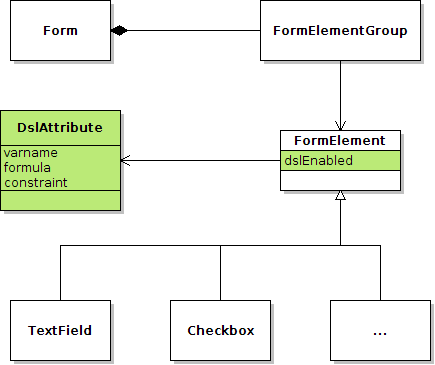
\includegraphics[scale=0.7]{figures/uml_datenmodell_neu}
\end{center}

\caption{Datenmodell der Formulare. Die grün gefärbten Bereiche sind jene, die im Zuge der Integration verändert wurden.}
\label{abb_uml_datenmodell}
\end{figure}

Jedes Formelement enthält eine boolesche Variable namens dslEnabled. Dieses Flag bestimmt, ob der Untertyp der Klasse Formelement zum Berechnen durch die FXL geeignet ist. Wenn ja, bekommt jedes Objekt dieses Formelements einen Verweis auf ein Objekt vom Typ DslAttribute. Die Klasse DslAttribute selbst enthält alle Informationen, die ein DSL-enabled Feld benötigt: den Variablennamen, eine Formel und einen Constraint. 

Es gibt zwei Möglichkeiten, die neue Klasse in das Datenmodell einzubinden: Als One-to-one Relation mit einem Foreign Key in einer der Klassen, oder als Embedded Object in der Klasse \texttt{Formelement}. In der ersten Variante wird eine eigene Tabelle für die Klasse \texttt{DslAttribute} erstellt. Über ein Id-Feld, welches zur Klasse hinzugefügt werden muss, wird die neue Tabelle über ein Foreign-Key Feld mit einem Formelement verbunden.

Die zweite Variante, die auch in der Implementierung verwendet wird, verändert lediglich die bestehende Tabelle der Formelemente. Es werden drei Spalten hinzugefügt, die die Attribute der Klasse \texttt{DslAttribute} repräsentieren. Der Vorteil dieser Methode ist, dass eine Tabelle weniger erstellt wird und somit ein Join bei der Abfrage eingespart wird.

\begin{lstlisting}[float = htbp,caption={Embedded DslAttribute },label=listing_dslattribute]
@Embeddable
public class DslAttribute {

  private FormElement formElement;
  
  @Column
  private String variableName;

  @Column
  private String formula;

  @Column
  private String constraintFormula;

  ...
}
\end{lstlisting}


Listing \ref{listing_dslattribute} enthält einen Auszug aus der neu erstellten Klasse, ohne Getter bzw. Setter und den Methoden toString(), hashCode() und equals().

\section{DSL Eingabe}
\label{implementierung_dsl_eingabe}

Die Eingabe des Variablennamens, der Formel und des Constraints erfolgt in der Eingabemaske des jeweiligen Formelements (siehe Abbildung \ref{abb_screenshot_spics_eingabe}). Dazu werden, wenn die DSL für den Typ des Formelements aktiviert ist, dem Eingabeformular drei Textfelder hinzugefügt, die per JSF an die Attribute der Klasse DslAttribute gebunden werden.


\begin{figure}[h]
\begin{center}
 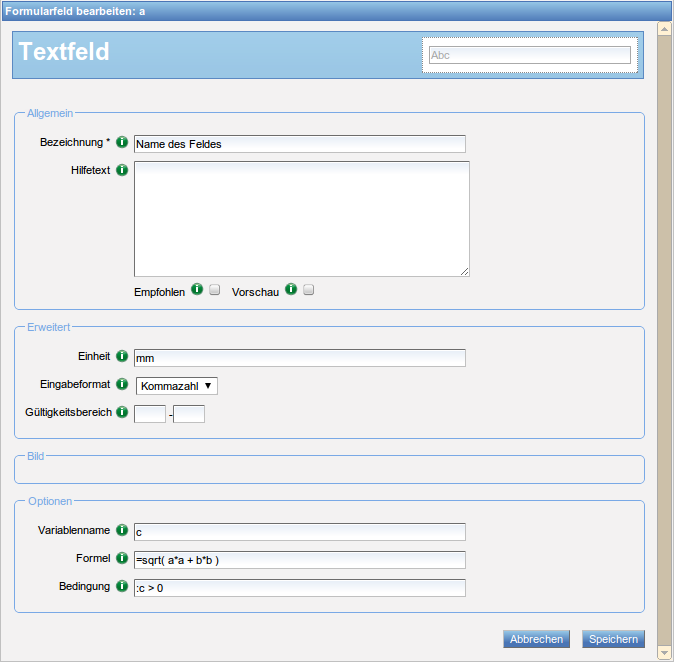
\includegraphics[scale=0.5]{figures/screenshot_spics_eingabe_neu}
\end{center}
\caption{Eingabe der DSL im Formulareditor}
\label{abb_screenshot_spics_eingabe}
\end{figure}

Hier wirft sich die Frage auf, ob es sinnvoll ist, die Angabe eines Constraints zu einem Feld, das durch eine Formel berechnet wird, zuzulassen. Meistens ist der Wert eines durch eine Formel berechneten Feldes ohnehin von anderen Feldern abhängig. Es erscheint also sinnvoll, die Validierung durch Constraints dort durchzuführen, um der Formel gültige Werte zu liefern. Andererseits muss eine Formel nicht von anderen Feldern abhängig sein\footnote{{Es kann durch Funktionen beispielsweise eine Formel erstellt werden, die einen Datumswert aus dem aktuellen Datum berechnet. Hier könnte ein Constraint der, z.B. vom Datum eines anderen Feldes abhängt, durchaus Sinn machen.}}. In der ersten Implementierung, die im Zuge dieser Arbeit durchgeführt wird, soll die Möglichkeit, ein Feld mit einer Formel und einem Constraint geichzeitig zu belegen, bestehen bleiben. Es bleibt zu evaluieren, inwieweit so eine Einschränkung, auch in Hinsicht auf eine Vereinfachung des User Interfaces und der damit eingehenden Verbesserung der Usability, sinvoll ist.

Beim Speichern wird ein Validator aufgerufen, der jedes der drei Felder gesondert validiert. Im Validator findet die Zyklenüberprüfung und die Überprüfung von Abhängigkeiten statt. Beim Speichern eines Formularelements sind mehrere Aspekte betreffend der DSL zu beachten:

\paragraph{Variablenname}
\begin{itemize}
	\item Der Variablenname darf nur einmal in dem Formular vorkommen.
	\item Der Variablenname darf nur aus Buchstaben und Ziffern bestehen, wobei das erste Zeichen ein Buchstabe sein muss.
	\item Um die Formeln nicht unübersichtlich werden zu lassen, wird die Länge der Variablen auf 15 Zeichen begrenzt.
\end{itemize}

\paragraph{Formel}
\begin{itemize}
	\item Alle Variablen, die in einer Formel verwendet werden, müssen bereits angelegt worden sein. Ein Anlegen der Variablen im Nachhinein soll nicht erlaubt werden, um die Konsistenz zu gewährleisten.
	\item Die Formeln eines Formulars dürfen keine zyklischen Abhängigkeiten enthalten (siehe Abschnitt \ref{implementierung_zyklenueberpruefung}).
	\item Die Formel darf sich nicht selbst referenzieren (also ein Verweis auf den Variablennamen des eigenen Feldes), da dies wiederum einer zyklischen Abhängigkeit entsprechen würde.
	\item Der Rückgabetyp der Formel muss dem Datentyp des Formelements entsprechen, da das Ergebnis der Formel sonst nicht zugewiesen werden kann.
\end{itemize}

\paragraph{Constraint}
\begin{itemize}
	\item Ein Constraint muss als Rückgabetyp Boolean haben, da er über die Gültigkeit der Eingaben entscheidet.
	\item Im Gegensatz zur Formel, darf sich ein Constraint auf den Wert des eigenen Feldes, sprich den eigenen Variablennamen beziehen. Dies ist not\-wen\-dig, um das eigene Feld zu validieren.
	
\end{itemize}

\section{Zyklenüberprüfung}
\label{implementierung_zyklenueberpruefung}

Ein essentieller Bestandteil der Validierung ist die Überprüfung auf zyklische Abhängigkeiten innerhalb eines Formulars. Diese Abhängigkeiten können als gerichteter Graph interpretiert werden: Enthält ein Formelement eine Formel mit Variablen, so sind alle Formelemente, die durch diese Variablen repräsentiert werden Nachfolger des Formularelements. Ist umgekehrt ein Formelement durch einen Variablennamen markiert, sind alle Formelemente, die eine Formel mit diesem Variablennamen enthalten, Vorgänger des Formelements. Abbildung \ref{abb_cycle_bmi_tree} zeigt den Graphen für das Beispielformular zur BMI-Berechnung.

\begin{figure}[ht]
\begin{center}
 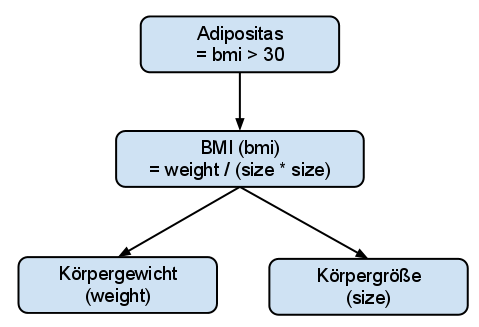
\includegraphics[scale=0.5]{figures/cycle_bmi_tree}
\end{center}
\caption{Baum der Abhängigkeiten im BMI-Formular}
\label{abb_cycle_bmi_tree}
\end{figure}

Die Interpretation der Abhängigkeiten als gerichteter Graph hilft bei der Überprüfung auf Zyklen. Ein Zyklus (oder Kreis) ist ein Weg von einem Knoten zu sich selbst \cite{Schl08}. Es gibt zwei grund\-sätz\-liche Algorithmen, die sich für die Überprüfung eignen: die Überprüfung durch Tiefensuche oder Breit\-en\-su\-che.

Die Tiefensuche ist ein Algorithmus, bei dem der Graph rekursiv abgearbeitet wird. Die bereits besuchten Knoten werden in einer globalen Liste abge\-spei\-chert. Wird ein Knoten besucht, der sich bereits in der Liste befindet, so liegt ein Zyklus vor. Durch Erweiterungen (Merken der Wege) können so alle Zyklen eines Graphen identifiziert werden.

Ein weniger mächtiger Algorithmus ist die Breitensuche. Diese ist ausreichend, wenn nur festgestellt werden soll, ob sich ein Knoten in einem Zyklus befindet oder nicht. Im Folgenden wird der Algorithmus zur Zyklenüberprüfung in der Implementierung (mittels Breitensuche) erläutert.

Die Eingabe ist das aktuelle Feld, das überprüft werden soll. Wenn keine Zyklen vorliegen, terminiert der Algorithmus. Wenn ein Zyklus gefunden wird, wird eine Exception geworfen. Ein Feld ist von einem anderen abhängig, wenn der Variablenname des Feldes in der Formel des anderen Feldes vorkommt.

\begin{enumerate}
  \item Überprüfe das aktuelle Feld, ob ein Variablenname und eine Formel vorhanden ist. Ist dies nicht der Fall, kann es nicht Teil eines Zyklus sein und die Überprüfung wird ohne Fehler beendet.
  
  \item Initialisiere die Menge \texttt{visited}. Sie enthält jene Felder, die bereits besucht wurden. 

  \item Füge den Variablennamen des aktuellen Feldes hinzu.

  \item Initialisiere die Menge \texttt{next}. Sie enthält jene Felder, die von den aktuell überprüften Feldern abhängen.

  \item Füge alle Variablen der Formel des aktuellen Feldes hinzu.

  \item Solange \texttt{next} nicht leer ist:

    \begin{enumerate}
      \item Wenn \texttt{visited} $\cup$ \texttt{next} $\neq$ \{\} : Es liegt ein Zyklus vor. Wirf Exception.
      \item Füge alle Elemente aus \texttt{next} zu \texttt{visited} hinzu.
      \item \texttt{next} = alle Nachfolger der Felder aus \texttt{next}.
    \end{enumerate}
\end{enumerate}


\section{Dateneingabe}
\label{implementierung_daten_eingabe}

Die Eingabe der medizinischen Daten in die Dokumentationssoftware ist der eigentliche Einsatzort der DSL. Hier werden die Formeln anhand der eingegebenen Daten berechnet und die Constraints überprüft. Vor der Implementierung werden allerdings einige Überlegungen benötigt, wie die Berechnung und Validierung der Werte durch die Aus\-führ\-ung der Formeln und Constraints am Besten umgesetzt wird.


\subsection{Aus\-führ\-ungszeitpunkt}

Ein Aspekt der Dateneingabe ist die Frage, wann die Formeln des Formulars ausgeführt werden. Im Beispiel des BMI-Rechners muss der BMI aus den Werten der Felder Kör\-per\-grö\-ße und Körpergewicht ausgerechnet werden. Es gibt mehrere Optionen, wann die Berechnung ausgelöst werden soll.

\begin{itemize}
	\item Beim Abspeichern eines Formulars: Die Felder, die durch Formeln berechnet werden, bleiben leer. Erst beim Speichern eines Formulars werden die abhängigen Felder berechnet. Wenn ein Fehler auftritt, wird der Benutzer zum Formular zurückgeleitet und aufgefordert, die Fehler zu beheben. Dies ist die ``sicherste'' Lösung, weil die asynchrone Kommunikation mit dem Server wegfällt. Diese Lösung ist allerdings nicht akzeptabel, da die Felder schon während des Ausfüllens berechnet werden sollen.

	\item In `Echtzeit' bei der Dateneingabe: Die Formeln werden nach der Eingabe eines Werts in ein Formularelement über einen Ajax-Validator berechnet. Der Eingabewert des Feldes wird nach der Eingabe\footnote{In der Implementierung wird, abhängig vom Typ des Eingabefeldes, entweder das \texttt{onblur}- oder \texttt{onchange}-Event des Formelements verwendet.} an den Server gesendet. Dort werden jene Felder, die vom eingegebenen Wert abhängen, berechnet und an den Client zurückgegeben, der die berechneten Werte in die ent\-sprech\-enden Felder einfügt.

	Die Möglichkeit der zusätzlichen wiederholten Berechnung nach dem Speichern bleibt allerdings bestehen.

	\item Auf Knopfdruck/Wunsch des Users: Die Werte der Felder werden nicht automatisch nach der Eingabe, sondern nur auf expliziten Wunsch des Users an den Server gesendet und dort berechnet. Zu\-sätz\-lich werden die Felder beim Speichern berechnet. Diese Lösung hätte den Vorteil, dass der Benutzer mehr Kontrolle über das Formular hat. Zu\-sätz\-lich werden etwaige Verzögerungen, die bei der `Echtzeit'-Lösung aufteten könnten vermieden.
\end{itemize}

In der Implementierung wurde der zweite Weg gewählt. Die Daten werden in Echtzeit an den Server gesendet und dort ausgewertet. Zu\-sätz\-lich werden die Felder noch einmal beim Speichern berechnet.

Die Frage der Auswertung stellt sich auch bei jenen Feldern, die mit Constraints belegt sind. Entweder werden die Constraints bereits beim Ausfüllen, oder erst beim Abspeichern evaluiert. Auch hier wurde eine Lösung aus beiden Möglichkeiten implementiert. 


\subsection{Aus\-führ\-ungsort}
\label{integration_ausfuehrungsort}

Webanwendungen bieten heutzutage dank Java\-Script die Möglichkeit, Berechnungen entweder clientseitig durchzuführen, oder das Ergebnis einer Berechnung mittels Ajax-Calls vom Server abzufragen und dann clientseitig weiter zu verarbeiten. Die Frage der client- oder serverseitigen Evaluierung der FXL stellt sich auch bei der Integration in SPICS.

\subsubsection{Clientseitige Evaluierung}

\begin{figure}[th]
\begin{center}
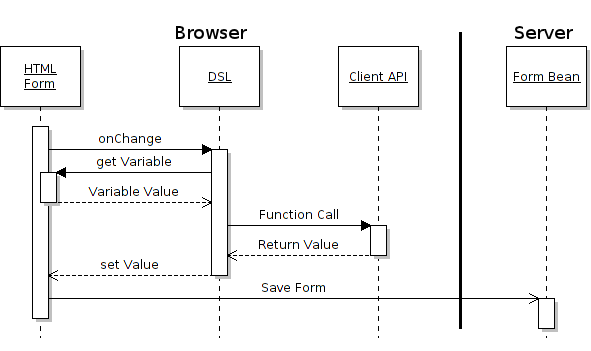
\includegraphics[scale=0.55]{figures/uml_seq_client_neu}
\end{center}

\caption{Clientseitige Lösung}
\label{abb_uml_seq_client}
\end{figure}


Grundsätzlich wäre eine clientseitige Evaluierung der Formeln möglich, indem man die DSL-Statements in Java\-Script übersetzt und im Browser ausführt. Die Übersetzung von FXL in Java\-Script ist möglich, da Java\-Script alle Sprachkonzepte, die FXL verwendet unterstützt\footnote{Tatsächlich das gleiche Verhalten wie Java\-Script zu erzeugen, ist nicht ganz so einfach, da Java\-Script bei manchen Operatoren ein anderes Verhalten an den Tag legt.}. Wenn eine Formel den Wert eines Feldes verändert, so wird dieser neue Wert im ent\-sprech\-enden Formularfeld gesetzt. Erst beim Speichern eines Formulars werden die berechneten und eingegebenen Werte an den Server gesendet, wo diese validiert und persistiert werden (Abbildung \ref{abb_uml_seq_client}).

Ein Schwachpunkt dieser Lösung ist, dass die in Java programmierten Funktionen, die in FXL verwendet werden können, nicht so einfach in Java\-Script übersetzt werden können wie die DSL-Statements selbst. Es ist also eine eigens für den Browser entwickelte API not\-wen\-dig, die alle Funktionen enthält, die der DSL auch am Server zur Verfügung stehen. Die Variablen können einfach aus den betreffenden Formularfeldern ausgelesen werden.

Eine Möglichkeit, den Overhead einer zusätzlichen clientseitigen Implementierung der Funktionen zu beseitigen, wäre die Weiterleitung der Funktionsaufrufe an den Server per Ajax-Call (Abbildung \ref{abb_uml_seq_client_hybrid}). Ein Bean am Applicationserver ruft die Methode in der Java-Implementierung auf und sendet den Rückgabewert zurück an den Browser. Der Nachteil ist, dass der Performance-Vorteil der clientseitigen Implementierung bei mehreren Funktionsaufrufen verloren geht.

\begin{figure}[h]
\begin{center}
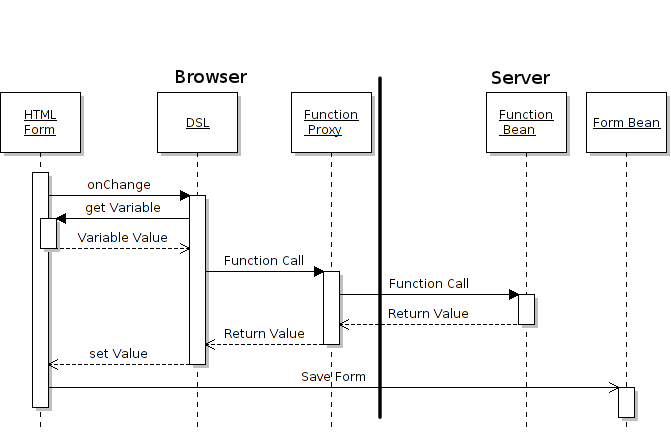
\includegraphics[scale=0.55]{figures/uml_seq_client_hybrid_neu}
\end{center}

\caption{Client- und serverseitige Hybridlösung}
\label{abb_uml_seq_client_hybrid}
\end{figure}

Ein weiterer Schwachpunkt der clientseitigen Lösung ist die Manipulierbarkeit von Skripten im Browser. Durch ent\-sprech\-ende Tools wie Firebug\footnote{http://getfirebug.com/}, können Nutzer das DOM und die Skripte manipulieren, und so eine korrekte Aus\-führ\-ung der DSL verhindern. Ein weiteres Defizit ist, dass die präzisen Fehlermeldungen, die für FXL definiert wurden, nun nicht nutzbar sind, da diese nicht in Java\-Script transferiert werden können.

\subsubsection{Serverseitige Evaluierung}

Die Alternative zur Evaluierung der Statements im Browser ist die Aus\-führ\-ung am Server (Abbildung \ref{abb_uml_seq_server}).

\begin{figure}[ht]
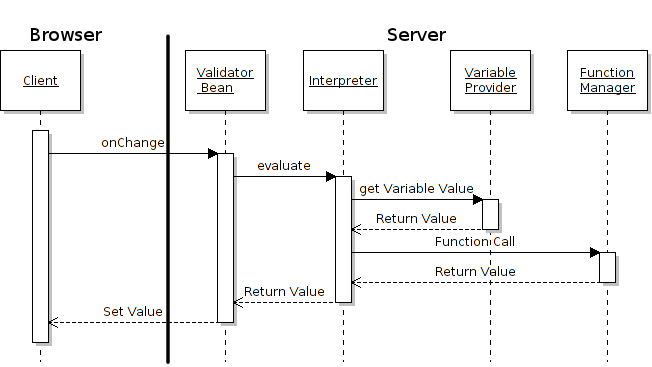
\includegraphics[scale=0.55]{figures/uml_seq_server_neu}
\caption{Aus\-führ\-ung am Server}
\label{abb_uml_seq_server}
\end{figure}

Das \texttt{onblur}- bzw. \texttt{onchange}-Event des Formularelements löst per JSF Ajax\-Support die Validierung des Formularelements am Applicationserver aus. Der eigens für die DSL implementierte DslValidator ruft die Komponente DslExecuter auf, die die DSL-Statements in korrekter hierarchischer Reihenfolge der Abhängigkeiten ausführt (vgl. Algorithmus in Abschnitt \ref{implementierung_integration_reihenfolge}). Für jede FXL-Formel wird ein Interpreter erstellt, der die Formel evaluiert und dabei auf die Implementierung des \texttt{VariableProvider} Interfaces und den Functionmanager zugreift. Zu\-sätz\-lich zu dem Feld, das das Event ausgelöst hat, werden auch die abhängigen Formularelemente neu gerendert.

Tritt bei der Aus\-führ\-ung der DSL-Statements ein Fehler auf, so wird eine ent\-sprech\-ende \texttt{FXLException} geworfen und über die Komponenten bis zum DslValidator weitergeleitet, wo diese abgefangen wird. Mithilfe des Fehlercodes wird eine FacesMessage erstellt und an den Context der Applikation übergeben. Diese Fehlermeldung wird im Browser beim betreffenden Formelement angezeigt.

Die serverseitige Lösung ist die einfachere Lösung, da die Aus\-führ\-ung einfach mittels FXL vorgenommen werden kann. Auch das Fehlerhandling erfolgt über die dafür vorgesehenen Exceptions, die dem Benutzer detailliertes Feedback geben. Bei der Integration im Zuge der praktischen Arbeit hat sich herausgestellt, dass die Antwortzeiten bei dieser Methode sehr gering sind. Ob die Verzögerung durch den Ajax-Call bei sehr komplexen Formularen eine unangenehme Verzögerung für den Benutzer darstellt, kann in einer weiteren Arbeit evaluiert werden. 


\subsection{Aus\-führ\-ungsreihenfolge}
\label{implementierung_integration_reihenfolge}

Die Aus\-führ\-ungsreihenfolge ist essentiell für die korrekte Auswertung der Formeln eines Formulars. Bevor ein Feld zur Berechnung herangezogen wird, muss sichergestellt werden, dass dieses selbst bereits berechnet wurde, wenn es eine Formel enthält. Wie bereits in Abschnitt \ref{implementierung_zyklenueberpruefung} erläutert, können die Abhängigkeiten in einem Formular als gerichteter zyklenfreier Graph gesehen werden. Wird ein Formularelement in der Formel eines anderen Elements verwendet, so kann dies als eine gerichtete Kante gedeutet werden.

Der folgende Algorithmus geht davon aus, dass keine Zyklen vorliegen. Die Zyklenfreiheit muss bereits beim Erstellen des Formulars sichergestellt werden (Abschnitt \ref{implementierung_zyklenueberpruefung}).

\begin{enumerate}
	\item Suche alle Felder, die einen Variablennamen, aber keine Formel beinhalten. Schreibe alle Werte der Felder in die Map \texttt{calculated<String, 			Result>}, wobei der Key der Variablenname ist und der Value der Wert des Feldes in einem \texttt{Result} Objekt.
	\item Erstelle eine Liste \texttt{formulas} aller Felder, die Formeln besitzen, sprich berechnet werden müssen.
	\item Solange \texttt{formulas} nicht leer ist, für jede Formel:
	
	\begin{enumerate}
		\item Hole alle Variablen aus der Tokenfolge der Formel.
		\item Wenn alle Variablen im KeySet von \texttt{calculated} sind:
		\begin{enumerate}
			\item Berechne die Formel.
			\item Wenn das Formelement der Formel einen Variablennamen hat, schreibe diesen mit dem berechneten Wert in \texttt{calculated}.
			\item Lösche die Formel aus \texttt{formulas}.
		\end{enumerate}	
		\item Wenn nicht alle Variablen bereits berechnet sind, ignoriere die Formel.
	\end{enumerate}	
	
\end{enumerate}

Der Algorithmus ist recht einfach: Zuerst werden alle Felder als berechnet angesehen, die selbst keine Formel beinhalten. Danach werden jene Felder berechnet, deren Formeln nur Variablen beinhalten, die auf bereits berechnete Felder verweisen. Durch die zugesicherte Zyklenfreiheit kann dieser Vorgang wiederholt werden, bis alle Felder berechnet sind.

Im Beispiel des BMI-Rechners (Abbildung \ref{abb_cycle_bmi_tree}) werden zuerst die Felder \emph{Körpergröße} und \emph{Körpergewicht} als berechnet markiert, da diese nicht von anderen Feldern abhängig sind. Danach werden die Felder mit Formeln, hier \emph{Adipositas} bzw. \emph{BMI}, in eine Liste ge\-spei\-chert, die in einer Schleife abgearbeitet wird. Wird zuerst versucht, das \emph{Adipositas}-Feld zu berechnen, wird festgestellt, dass das Feld \emph{BMI} noch nicht berechnet wurde und der Versuch verworfen. Danach wird das Feld \emph{BMI} aus den Feldern \emph{Körpergröße} und \emph{Körpergewicht} berechnet und aus der Liste entfernt. Beim nächsten Schleifendurchlauf kann nun die Formel der \emph{Adipositas}-Checkbox ausgewertet und aus der Liste gelöscht werden.

Bei der Aus\-führ\-ung wirft sich die Frage auf, wie vorgegangen werden soll, wenn ein Eingabefeld mit Variablenname noch nicht ausgefüllt wurde. In diesem Fall liefert die \texttt{lookup()}-Methode des \texttt{VariableProvider} ein \texttt{Result}-Objekt vom richtigen Datentyp, aber mit Wert \texttt{null} zurück. Die ganze Formel wird, wie im Abschnitt \ref{design_interpreter} beschrieben, zu einem \texttt{Result}-Objekt mit Wert \texttt{null} ausgewertet. Ist ein Feld also noch leer, werden auch die abhängigen Felder nicht mit einem Wert belegt. Wichtig ist jedoch, dass die Aus\-führ\-ung nicht unterbrochen wird und alle Felder, die nicht von einem nicht ausgewerteten Feld abhängen können, berechnet werden.



\section{Fehlerbehandlung}
\label{integration_fehlerbehandlung}

Durch die sehr detaillierten Fehlermeldungen der DSL-Implementierung ist es möglich, dem Benutzer ein genaues Feedback zu geben, wenn Probleme auftreten. Zu\-sätz\-lich zu den vorgegebenen Fehlern ist es sinnvoll, auch implementierungsspezifische Fehlermeldungen zu definieren.

Wenn Exceptions bei der statischen Analyse oder der Aus\-führ\-ung eines Statements auftreten, so müssen diese intelligent weitergeleitet und an der richtigen Stelle im System abgefangen werden, um einen reibungslosen Ablauf des Workflows zu ermöglichen, aber vor allem um den ordnungsgemäßen Betrieb des Systems nicht zu gefährden.

\subsection{Implementierungsfehler}

In der Dokumentationssoftware können Fehler an zwei Stellen auftreten: Bei der Modellierung eines Formulars und bei der Aus\-führ\-ung der Formeln und Constraints beim Ausfüllen eines Formulars. Jene Fehler, die beim Ausfüllen auftreten, wie etwa eine Division durch null, werden bereits von den in Abschnitt \ref{section_design_fehlerbehandlung} definierten Implementierungsfehlern abgedeckt. Wenn eine ent\-sprech\-ende \texttt{FXLException} geworfen wird, wird diese am Server abgefangen. Anhand des Fehlercodes wird die ent\-sprech\-ende internationalisierte Nachricht erstellt (siehe unten). 


\begin{table}
\begin{tabular}[ht]{|c | p{11cm}|}
	\hline
	\textbf{Code} & \textbf{Beschreibung}\\
	\hline
  	\hline
  	4xx  & \multicolumn{1}{|l|}{\textsc{Implementierungsfehler}} \\
  	\hline
  	400  & Allgemeiner/unbekannter Implementierungsfehler    \\
  	\hline
  	411  & Ungültiger Variablenname    \\
  	\hline
  	412  & Variablenname zu lang    \\
  	\hline
  	413  & Variablenname bereits vorhanden   \\
  	\hline
  	414  & Die Formel erzeugt zyklische Abhängigkeiten    \\
  	\hline
  	415  & Die Formel enthält unbekannte Variablen    \\
  	\hline
  	416  & Rückgabetyp der Formel stimmt nicht mit Datentyp des Formelements überein    \\
  	\hline
  	417  & Rückgabetype eines Constraints ist nicht Boolean    \\
  	\hline
\end{tabular}
\caption{Fehlercodes für Implementierungsfehler}
\end{table}

Neu und spezifisch für den Einsatzbereich der DSL sind jene Fehler, die beim Erstellen der Formulare auftreten. Diese decken vor allem Fehler des Formats von Variablen, der logischen Struktur der Abhängigkeiten und der Rückgabetypen ab.



\subsection{Internationalisierung}

Die Internationalisierung der Fehlermeldungen erfolgt mit ``Boardmitteln'' von Seam\footnote{ vgl. http://docs.jboss.org/seam/latest/reference/en-US/html/i18n.html, 21.12.2011}. Die Labels werden in Properties-Files für alle unterstützten Sprachen ge\-spei\-chert (Listing \ref{listing_error_de} bzw. \ref{listing_error_en}).

\begin{lstlisting}[float = htbp,caption={Deutsche Fehlermeldungen },label=listing_error_de]
error.dsl.202=Ungueltige Kombination von Typen fuer Operator {0}: {1}, {2}
error.dsl.211=Variable nicht gefunden: {0}
error.dsl.212=Variable mehrfach definiert: {0}
\end{lstlisting}

\begin{lstlisting}[float = htbp,caption={Englische Fehlermeldungen},label=listing_error_en]
error.dsl.202=Invalid type combination for operator {0}: {1}, {2}
error.dsl.211=Variable not found: {0}
error.dsl.212=Variable defined more than once: {0}
\end{lstlisting}

Zur Identifizierung der Labels wird der Fehlercode der Exception verwendet. Um das Feedback duch fehlerspezifische Informationen anzureichern, werden die Argumente der Fehlermeldungen, wie in Listing \ref{listing_error_de} bzw. \ref{listing_error_en} ersichtlich verwendet.




